\documentclass[10pt, a4paper]{article}
%\documentclass[10pt, twocolumn, a4paper]{article}
\usepackage{listings}
\usepackage{pdfpages}
\usepackage[legalpaper, margin=1in]{geometry}

%------------------------------------------------------------------------------------
\begin{document}
\begin{titlepage}
   \begin{center}
       \vspace*{1cm}
       \large
       \textbf{Homework 1: Introduction to Algorithmic Analysis and Recurrence}
       \normalsize

       \vspace{0.5cm}

       \textbf{Author: Gabriel Hofer}

       \vspace{0.5cm}

       CSC-372 Analysis of Algorithms

       \vspace{0.5cm}

       Instructor: Dr. R

       \vspace{0.5cm}

       Section 1 DUE: Thursday, Aug 27th, at 7AM  \newline
       Section 2 DUE: Thursday, Sept 3 th, at 7AM  

       \vfill

       Department of Computer Science and Engineering\\
       South Dakota School of Mines and Technology\\

   \end{center}
\end{titlepage}
%------------------------------------------------------------------------------------
\newpage
\textbf{Introductory Information}

\begin{enumerate}

  \item (3 pt) How soon do you need to notify me for a normal extension? \\
    \textbf{36 hours}

  \item (3 pt) How many projects will there be? \\
    \textbf{5 projects}

  \item (3 pt) How long do you have to notify me for a possible grading error, starting when? the grade \\
    \textbf{One week}

  \item (3 pt) What is the ONLY option to bring up your grade at the end of the semester? \\
    \textbf{Take the optional second chance Exam}

  \item (8 pt) When did you attend ZOOM office hours after Aug 19 (this will confirmed later)? \\
    \textbf{August 21, 2020  }

  \item (3 pt) Should your microphones/video initially be on or off when attending a Zoom recitation/office hours. \\
    \textbf{Start with camera and microphone off.}

  \item (3 pt) What topic(s) are tentatively planned for Oct. 9? \\
    \textbf{F: Closest Pair of points}

  \item (3 pt) At minimum view, the entry quiz (competition is not required) \\
    \textbf{Check-in Completed}

    %  ------------------------End: Graded all or nothing------------------------------------------
  \item 9. (6 pt) What is the run time for the following code. You MUST show your work for any credit \\ 

  \begin{lstlisting}
  Let A be an array of size n
  for a in the range of 1 to x
      for b in the range of 1 to y
          for c in the range of 1 to z
              print all of A

  \end{lstlisting}

  The outer loop executes x times. The first nested loop executes y times. 
    The second nested loop executes z times. Printing all of A requires n operations.
    Because these loops are all nested, we multiply their run times together. 

  Runtime = $ O(x) * O(y) * O(z) * O(n) $

  Runtime = $ O(x * y * z * n) $

    \section{a.}

  \textbf{Insertion Sort: }
  \begin{lstlisting}
    vector<int> insertionSort(vector<int> & v) {
        int key, i;
        for (int j = 1; j < v.size(); j++) {
            key = v[j];
            i = j - 1;
            while (i >= 0 && v[i] > key) {
                v[i + 1] = v[i];
                i--;
            }
            v[i + 1] = key;
        }
        return v;
    }
  \end{lstlisting}

  \textbf{Merge Sort:}
  \begin{lstlisting}
    vector<int> mergeSort(vector<int> v) {
        if (v.size() > 1) {
            vector<int> left((v.size() + 1) / 2);
            vector<int> right(v.size() - left.size());
            for (int i = 0; i < (v.size() + 1) / 2; i++) 
                left[i]=v[i];
            for (int i = 0; i < v.size()-left.size(); i++) 
                right[i]=v[i+left.size()];
            left = mergeSort(left);
            right = mergeSort(right);   
            int l = 0, r = 0;
            while (l<left.size() && r<right.size()) {
                if (left[l] <= right[r]) {
                    v[l+r] = left[l];
                    l++;
                } else {
                    v[l+r] = right[r];
                    r++;
                }
            }
            while (l < left.size()) {
                v[l + r] = left[l];
                l++;
            }
            while (r < right.size()) {
                v[l + r] = right[r];
                r++;
            }
        }
        return v;
    }
  \end{lstlisting}

  \section{b.}

  \section{c. }
  \subsection{a. OUTPUTing runtimes}b

  \subsection{Tables}
  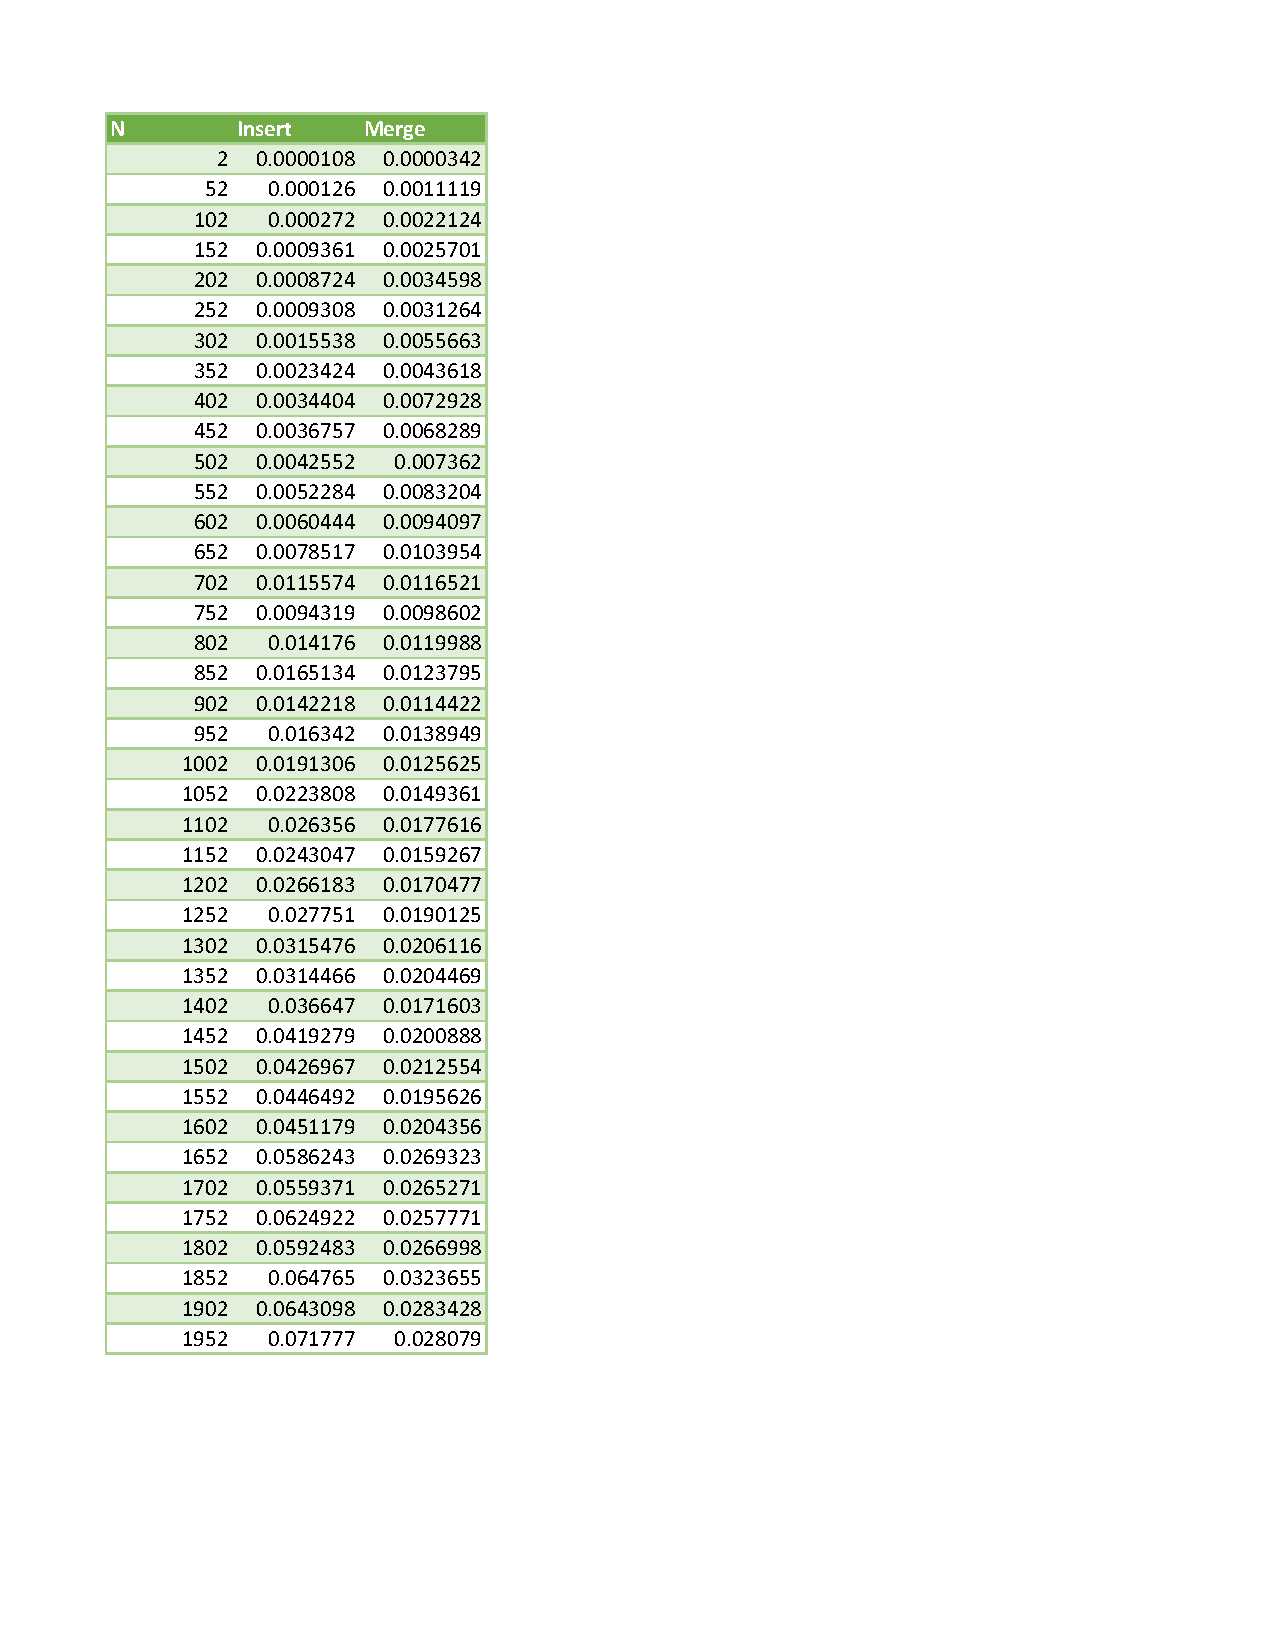
\includepdf[scale=.8,pages=-,pagecommand=\subsection{Insertion Sort vs Merge Sort for Small N}]{smallNtable.pdf}
  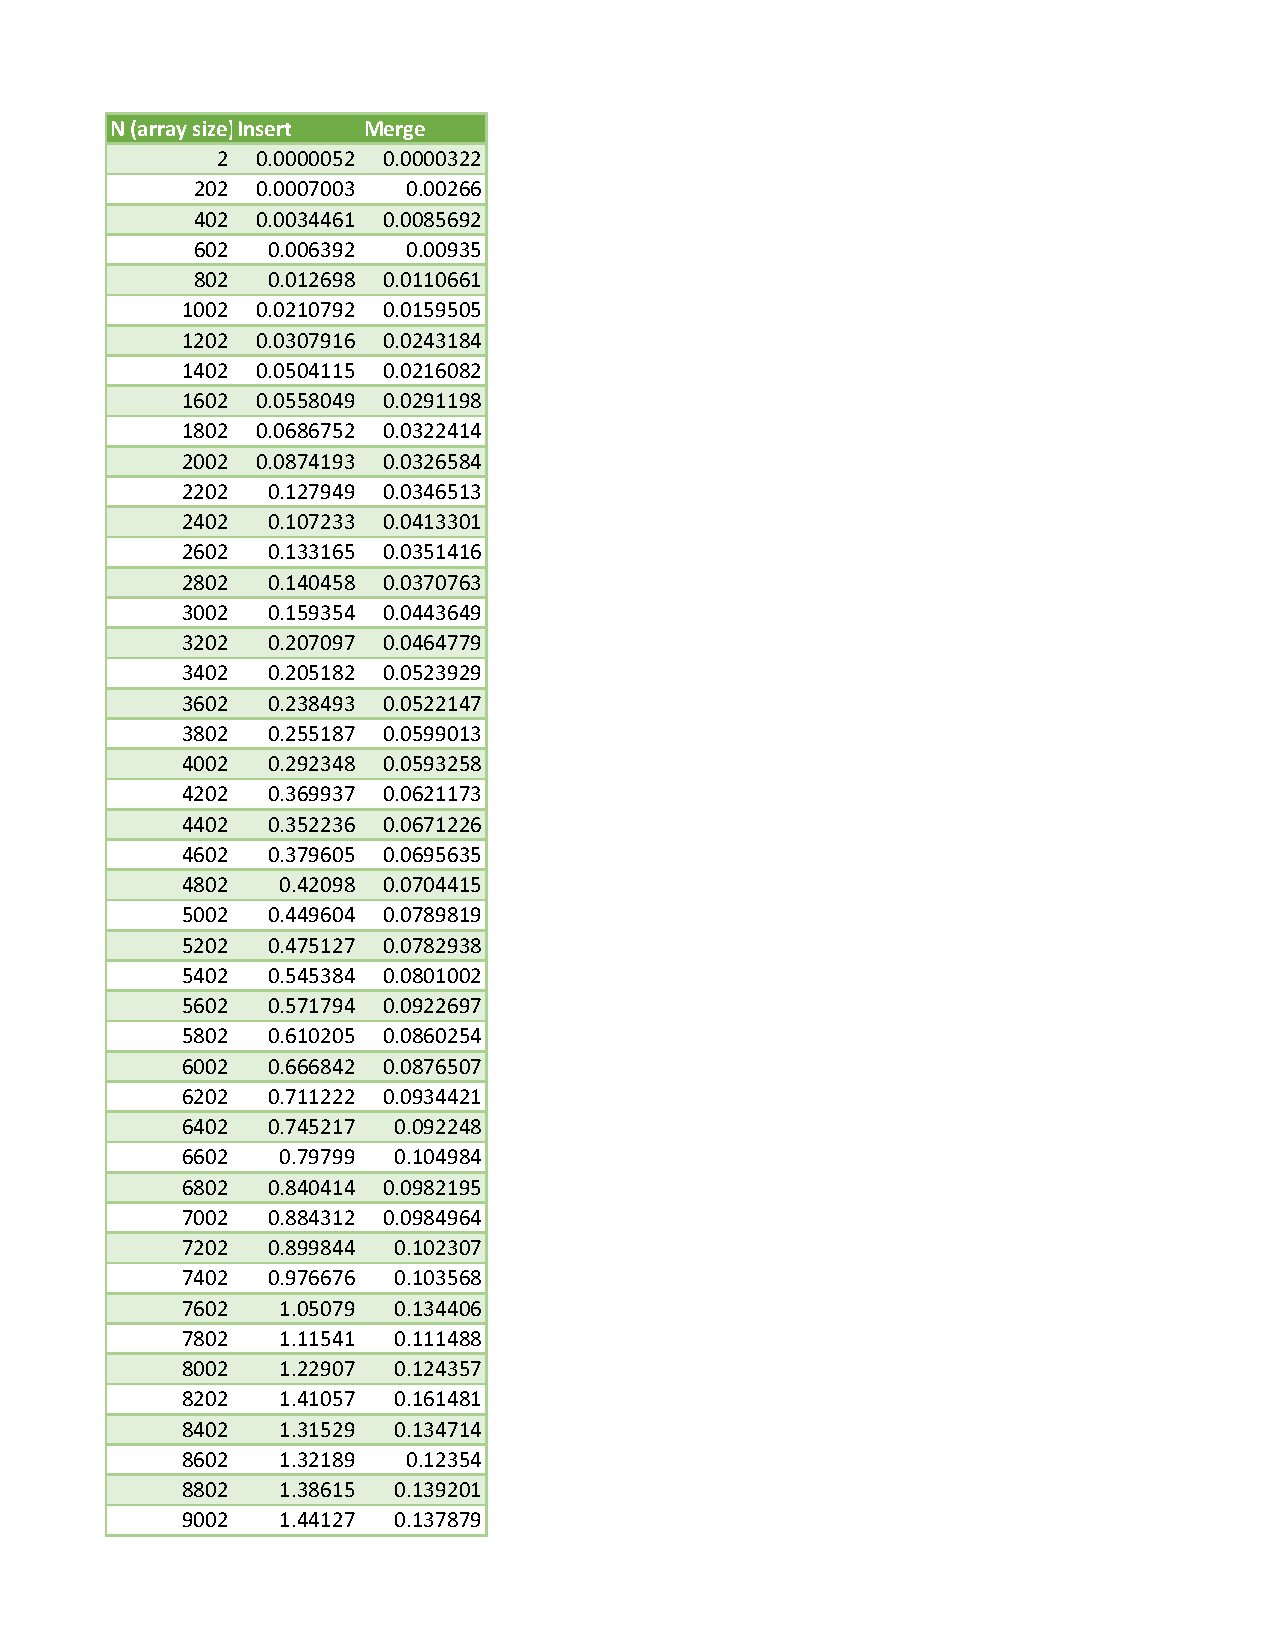
\includepdf[scale=.8,pages=-,pagecommand=\subsection{Insertion Sort and Merge Sort for Large N}]{largeNtable.pdf}
    \section{d. Charts}
  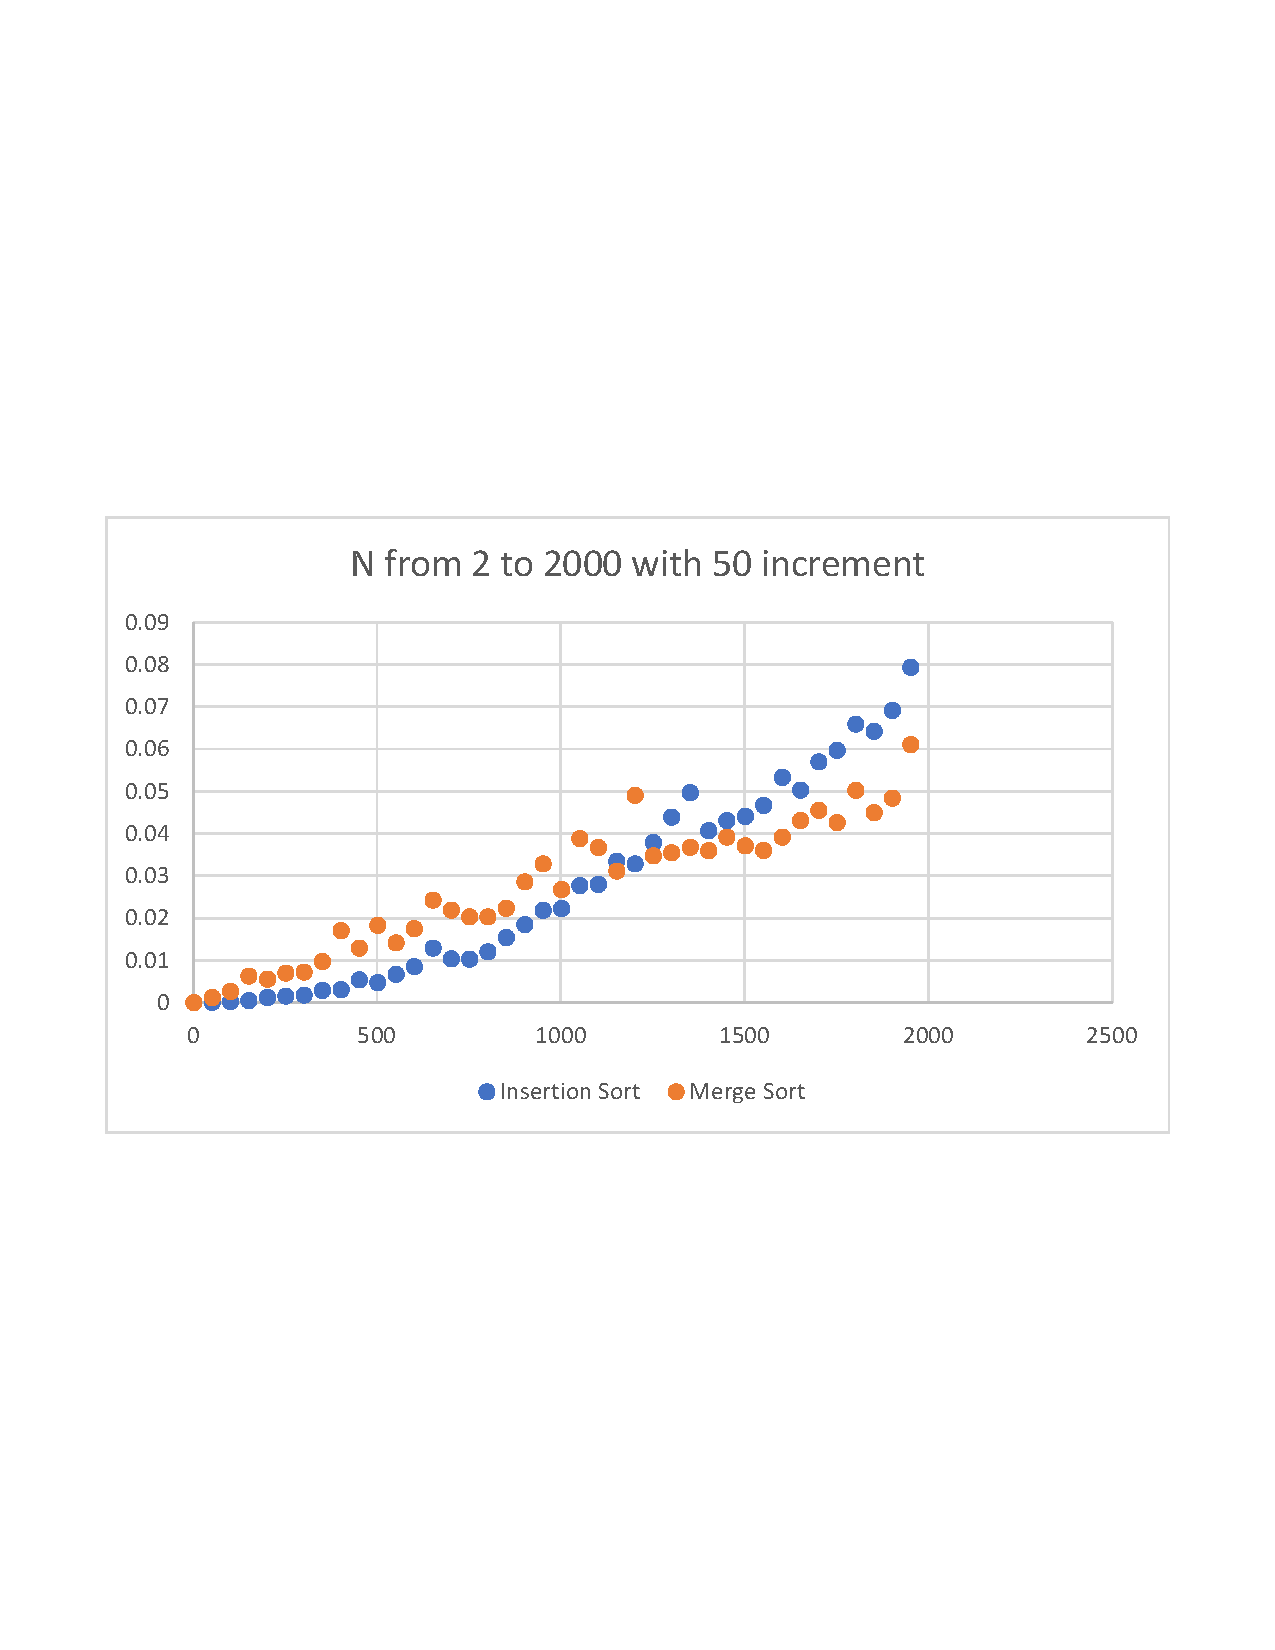
\includepdf[scale=1,pages=-]{smallNchart.pdf}
  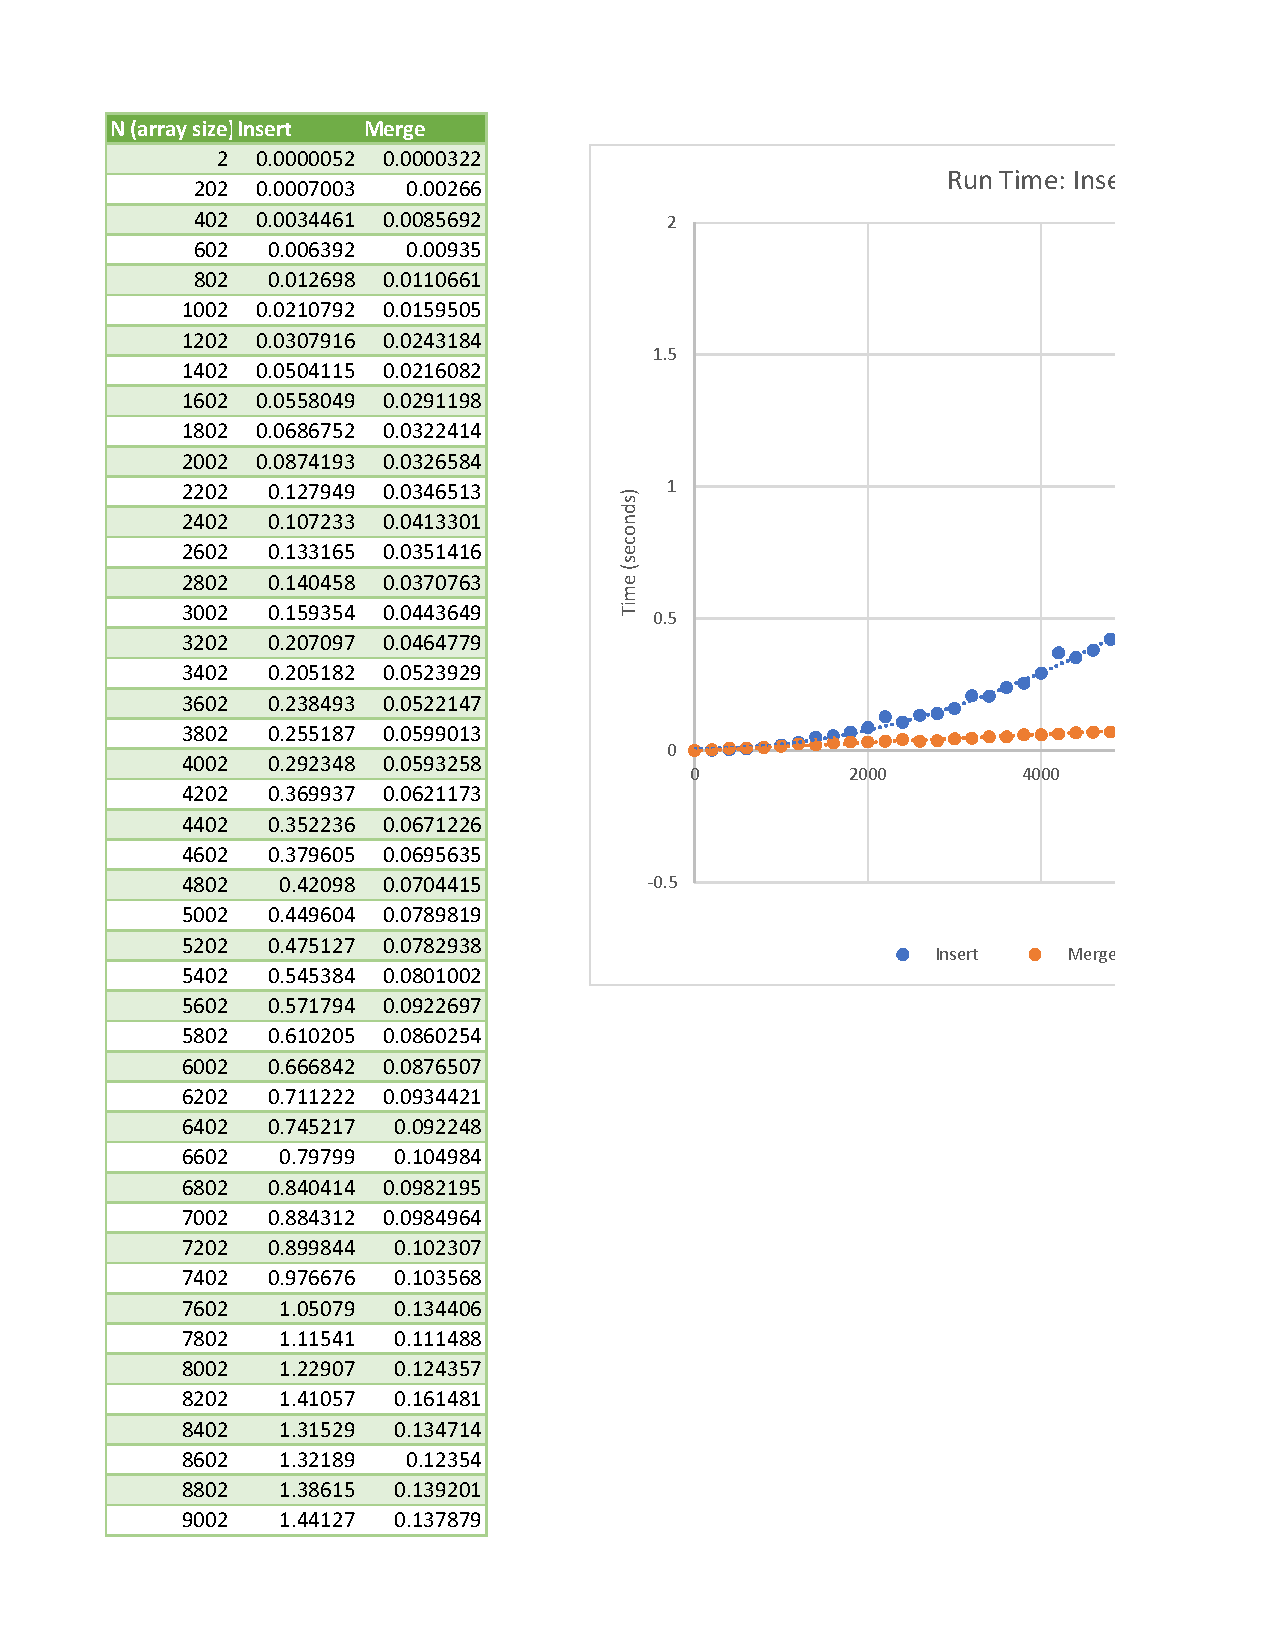
\includepdf[scale=1,pages=-]{largeNchart.pdf}
  % \section{Analysis}

\end{enumerate}

\end{document}









